\chapter{Baseline}
\label{chap:baseline}


	% --- META INFO START: ---

	\besk{ Mellomkapittel om allerede-eksisterende approaches og teori jeg brukte som starting point og som jeg verifiserer og sammenlikner med senere }

	% --- META INFO STOP. ---


Kristian Nymoen et al. \cite{nymoen_synch} showed how one can, by amongst other measures endowing oscillators with self awareness capabilities, achieve synchronization (\textit{harmonic} at that, cf. \ref{subsec:harmonic_synchrony}) of pulse coupled oscillators while synchronizing both phases and frequencies.

Other than endowing their firefly oscillators with self awareness capabilities, they developed update functions for both phases and frequencies which cause (close to) 0 change half-way through the oscillator cycle. These (close to) 0 changes half-way through robots's oscillator cycles enable individual musical robots to play e.g. half as quickly as other individuals—which typically characterizes musical interaction—as well as the possibility of achieving the target state of harmonic synchrony. Their contribution also differs from previous approaches in that Nymoen et al.'s fireflies only need to transmit ``fire'' signals every other phase climax, not every single phase climax. 

The aforementioned update functions, as well as how additional self awareness capabilities are incorporated in one of them, are now presented in \ref{subsec:nymoen_phase_adjust} and \ref{subsec:nymoen_freq_adjust}. Then, the relatively new system target state of \textit{harmonic synchrony} will be expounded and explained in \ref{sec:harmonic_synchrony}.



\section{Phase synchronization} % or adjustment
\label{sec:nymoen_phase_updates}


% --- META INFO START: ---

\gjor{ Introduser det første phase ($\phi$) synchronization problemet, uthevet og i fet skrift. Deretter fortsett til løsningene dens (Phase-Adj.-metodene). "This is the first and simpler problem to solve, namely synchronizing the phases $\phi_i$ of all agents $i$." }

% --- META INFO STOP. ---


	\subsection{Mirollo-Strogatz's ``standard'' phase adjustment} % or phase synchronization, or phase updates
	\label{mirollo_strogatz_phase_adjust}
	
	% --- META INFO START: ---
	
		\gjor{ Muligens inkluder introen i Section \ref{sec:phase_methods} her også (eller bare her?) }
	
	% --- META INFO STOP. ---
	
	One approach having been used to achieve this in the past is Mirollo-Strogatz's ``Standard'' phase-adjustment in oscillators \cite{mirollo_strogatz_PCO_synch}.
	
	Each musical agent gets a new phase, $\phi(t^+) = P(\phi(t))$, accoring to the \textbf{phase update function \eqref{strog_phase}} upon perceiving a ``fire''-event from one of the other musical nodes:
	
	\begin{equation}
	\label{strog_phase}
		\phi(t^+) = P(\phi(t)) = (1 + \alpha)\phi(t) ,
	\end{equation} \nl
	where $\alpha$ is the pulse coupling constant, denoting the strength between nodes \cite{nymoen_synch}, $t^+$ denotes the time-step immediately after a ``fire''-event is heard, and $\phi(t)$ is the old frequency of the agent at time $t$. 
	
	So, if e.g. $\alpha = 0.1$, then a musical agent's new and updated phase, immediately after hearing a ``fire''-signal from another agent, will be equal to $\phi(t^+) = P(\phi(t)) = (1 + 0.1)\phi(t) = 1.1\phi(t)$. 110\% of its old phase $\phi(t)$, that is. Hence, and in this way, the agent would be ``pushed'' to fire sooner than it would otherwise (as nodes fire once they have reached phase-climax $\phi(t)=1$).


	\subsection{K. Nymoen's bi-directional phase adjustment} % or 'shifts', as used before.
	\label{subsec:nymoen_phase_adjust}

	This approach to phase-adjustment works very similarly to the phase-adjustment performed in the ``standard'' \textbf{\textit{Mirollo-Strogatz}} approach presented earlier; the only difference being that now, nodes update their phases with the slightly more complex \textbf{phase update function \eqref{nymoen_phase}} when hearing a ``fire''-event from one of the other musical nodes — allowing for both larger, but also smaller, updated phases compared to the old phases:

	\begin{equation}
	\label{nymoen_phase}
		\phi(t^+)=P(\phi(t)) = \phi(t) - \alpha \cdot sin(2\pi\phi(t)) \cdot | sin(2\pi\phi(t)) | ,
	\end{equation} \nl
	where $t^+$ denotes the time-step immediately after a ``fire''-event is heard, and $\phi(t)$ is the old frequency of the agent at time $t$.

	The fact that new and updated phases can both be larger, but also smaller, compared to the old phases, is exactly what's meant by the phase-adjustment being \textbf{\textit{bi-directional}}, or as the authors call it in the paper as using both excitatory and inhibitory phase couplings between oscillators \cite{nymoen_synch}.

	The effects then of adjusting phases—upon hearing ``fire''-events, according to this newest update-function \eqref{nymoen_phase}—are that the nodes's updated phases $\phi(t^+)$, compared to their old phases $\phi(t)$, now get decreased if $\phi(t)$ is lower than 0.5, increased if $\phi(t)$ is higher than 0.5, and neither—at least almost—if the phases are close to $0.5$. This is due to the negative and positive sign of the sinewave-component in Equation \eqref{nymoen_phase}, as well as the last attenuating factor in it of $| sin(2\pi\phi) | \approx | sin(2\pi \frac{1}{2}) | = | sin(\pi) | = | 0 | = 0$, then if we have $\phi(t) \approx 0.5 = \frac{1}{2}$.

% --- \section END. ---



\section{Phase \& frequency synchronization}


% --- META INFO START: ---

\gjor{ Introduser det andre, og mer utfordrende, phase \& frequency ($\phi$-\&$\omega$) synchronization problemet, uthevet og i fet skrift. Deretter løsningene dens (Freq.-Adj.-metodene), som man må bruke i tillegg til $\phi$-løsningene eller Phase-Adjustment-metodene. "This is the second and harder problem of synchronizing both phases $\phi_i$, as well as frequencies $\omega_i$, for all agents $i$ more or less simultaneously." }

% --- META INFO STOP. ---

Only one frequency adjustment / update function was used as a starting point for this thesis and eventually implemented in the Unity synchrony simulator. This one frequency synchronization method, as invented by Nymoen et al. \cite{nymoen_synch}, is now presented. \nl

\textbf{K. Nymoen's frequency adjustment} \nl
This approach to frequency adjustment stands in contrast to previous approaches to synchronization in oscillators [fixed\_freqs, fixed\_range\_freqs] where the oscillators's frequencies are either equal and fixed, or where frequencies are bound to initialize and stay within a fixed interval/range.

In order to achieve this goal of \textit{harmonic synchrony} in conjunction with|or rather through|frequency adjustment, we have to go through a few steps to build a sophisticated enough update-function able to help us achieve this.

When it comes to the temporality and timing of when these update functions are used and applied; Musical agents's phases get updated/adjusted immediately as ``fire''-/``flash''-events are perceived, whereas agents's frequencies do not get updated until the end of their oscillator-cycle (i.e. when having a phase-climax $\phi(t)=1$). This is also the reason why frequencies are updated discretely, not continuously. So-called H-values however, being ``contributions'' with which the frequencies are to be updated according to, are immediately calculated and accumulated when agents are perceiving a ``fire''-/``flash''-event — and then finally used for frequency-adjustment/-updating at phase-climaxes.
		
Each agent $i$ update their frequency, on their own phase-climax (i.e. when $\phi_i(t)=1$), according to the frequency-update function $\omega_i(t^+)$:

\begin{equation}
	\omega_i(t^+) = \omega_i(t) \cdot 2^{F(n)},
\end{equation}

where $t^+$ denotes the time-step immediately after phase-climax, $\omega_i(t)$ is the old frequency of the agent at time $t$, and $F(n) \in [-1,1]$ is a quantity denoting how much and in which direction an agent should update its frequency after having received its $n$th ``fire''-signal.

This is how we obtain the aforementioned $F(n)$-quantity:

	\paragraph{Step 1: the ``in/out-of synch'' error-measurement/-score, $\epsilon(\phi(t))$}

	Describing the error measurements at the n-th ``fire''-event, we introduce an Error Measurement function.

	The error measurement function \eqref{error_measurement}, plotted in Figure \ref{fig:error_measurement}, is calculated immediately by each agent $i$, having phase $\phi_i(t)$, when a ``fire''-event signal from another agent is detected by agent $i$ at time $t$.

	\begin{equation}
	\label{error_measurement}
		\epsilon(\phi_i(t)) = sin^2(\pi\phi_i(t))
	\end{equation} \nl

	\begin{figure}[ht!]
		\centering
		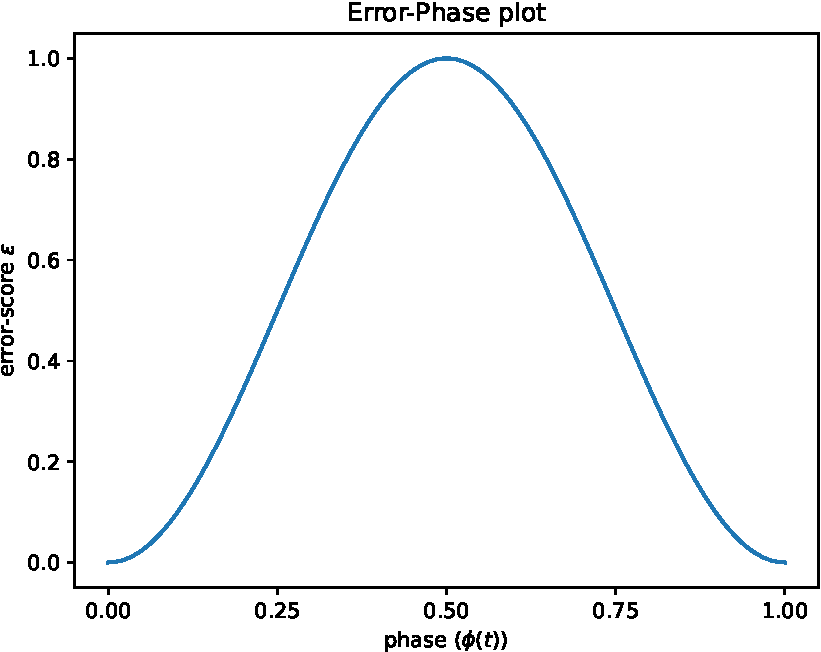
\includegraphics[width=0.65\linewidth]{Assets/DocSegments/Chapters/Baseline/Figures/Functions/PhaseErrorFunction.pdf}
		\caption[Plot of error-measurement function for K. Nymoen's frequency-adjustment]{Error measurement \eqref{error_measurement} plotted as a function of phase}
		\label{fig:error_measurement}
	\end{figure}

	As we can see from this error-function, the error-score is close to 0 when the agent's phase $\phi_i(t)$ is itself close to 0 or 1 (i.e. the agent either just fired/flashed, or is about to fire/flash very soon). This implies that if it was only short time ago since we just fired, or conversely if there is only short time left until we will fire, we are not much in error or \textit{out-of-synch}. 

	The error-score is the largest when an agent perceives a ``fire''-signal while being half-way through its own phase (i.e. having phase $\phi(t)=0.5$). We could also then ask ourselves, does not this go against the main/target goal of the system, being \textit{harmonic synchrony} — if agents are allowed to be ``half as fast'' as each other? We could imagine a completely ``legal'' and harmonically synchronous scenario where two agents have half and double the frequency of each other. The agent with half the frequency of the faster agent would then have phase $\phi(t)=0.5$ when it would hear the faster agent ``fire''/``flash'' — leading to its Error-score $\epsilon(0.5) = sin^2(\pi/2) = 1$, which then makes it seem like the slower agent is maximally out of synch, when it is actually perfectly and harmonically synchronized. This calls out for an attenuating mechanism in our frequency update function, in order to ``cancel out'' this contribution so that perfectly harmonically synchronized agents will not be adjusted further despite their high Error-measurement. As we will see below, in Figure \ref{fig:rho_n}, exactly such an attenuating mechanism is utilized in our frequency-adjustment method.

	This error-measurement/-score forms the basis and fundament for the first component of self-awareness, being the \textit{self-assessed synchrony-score} $s(n)$.


	\paragraph{Step 2: The first self-awareness component, s(n)}
	\label{s_n}
	This aforementioned self-assessed synchrony-score, $s(n)$, is in fact simply the median of error-scores $\epsilon$.

	If we then have a high $s(n)$-score, it tells us that the median of the $k$ last error-scores is high, or in other words that we have mainly high error-scores — indicating that this agent is out of synch. Conversely, if we have a low $s(n)$-score, indicating mainly low error-scores for the agent — then we have an indication that the agent is in synch, hence leading to low error scores, and in turn low $s(n)$-scores. 

	In other words, each agent hence has a way to assess themselves in how much in- or out-of-synch they believe they are compared to the rest of the agents. This is then the first degree/aspect of \opphoy{public} self-awareness in the design.

	\paragraph{Step 3: frequency update amplitude- \& sign-factor, $\rho(n)$}

	Describing the amplitude and sign of the frequency-modification of the n-th ``fire-event'' received. It is used to say something about in which direction, and in how much, the frequency should be adjusted.

	\begin{equation}
	\label{amp_sign_freq_adj}
		\rho(\phi) = - sin(2\pi\phi(t)) \in [-1, 1]
	\end{equation}

	\begin{figure}[ht!]
		\centering
		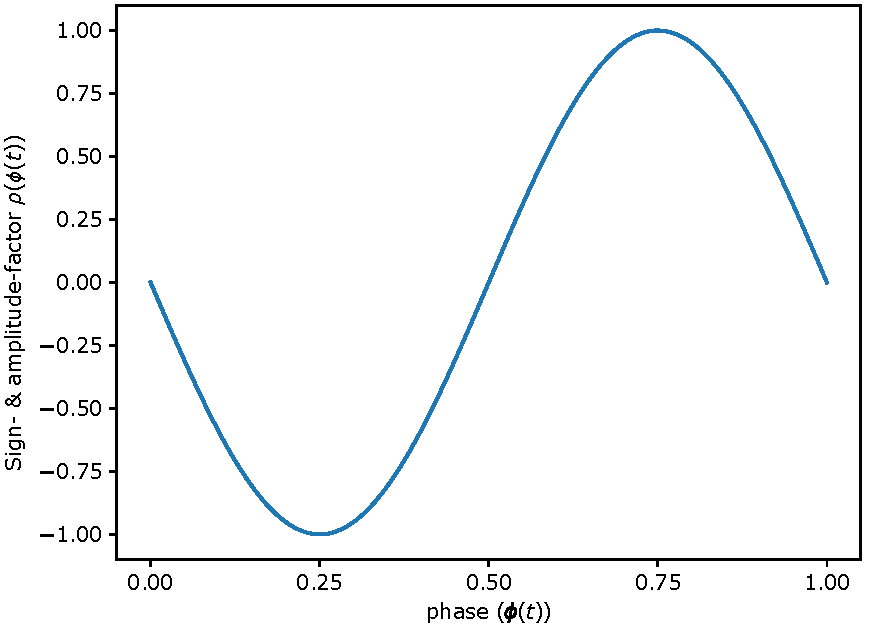
\includegraphics[width=0.65\linewidth]{Assets/DocSegments/Chapters/Baseline/Figures/Functions/rho_n.pdf}
		\caption[Plot of amplitude- \& sign-factor for K. Nymoen's frequency-adjustment]{The amplitude- \& sign-factor, $\rho(\phi(t))$, where $\phi(t)$ is the phase of an agent at time $t$ when it heard ``fire''-event $n$. Notice how the amplitude is equal to 0 when the phase is equal to 0,5.}
		\label{fig:rho_n}
	\end{figure}

	For example, if an agent $i$ has phase $\phi_i(t)=1/4$, it gets a value $\rho(1/4) = - sin(\pi/2) = -1$; meaning, the agent's frequency should be decreased (with the highest amplitude actually) in order to "slow down" to wait for the other nodes. Conversely, if an agent $j$ has phase $\phi_j(t)=3/4$, it gets a value $\rho(3/4) = - sin(3/2 \pi) = -(-1) = 1$; meaning, the agent's frequency should be increased (with the highest amplitude) in order to getting "pushed forward" to catch up with the other nodes.

	Acts as an attenuating factor, when $\phi(t)\approx0.5$, in the making of the H-value — supporting the goal of \textit{harmonic synchrony}.
	

	\paragraph{Step 4: the H-value, and the H(n)-list}
	\label{H_n}

	The following value, being ``frequency-update-contributions'', is then (as previously mentioned) calculated immediately when the agent perceives another agent's ``flashing''-signal:

	\begin{equation}
	\label{h_value}
		H(n) = \rho(n) \cdot s(n)
	\end{equation}

	Here we then multiply the factor $\rho(n)$, depicted in Figure \ref{fig:rho_n}, representing how much, as well as in which direction, the agent should adjust its frequency, together with a factor $s(n) \in [0,1]$ of the adjusting agent's self-assessed synch-score. This means that all the possible values this $H(n)$-value can take, lies within the green zone in Figure \ref{fig:all_possible_H_n_values}. We hence see that the smallest value $H(n)$ can take for the $n$th ``fire''-event is -1, which it does when $\phi(n) = 0.25$ and $s(n) = 1$. The highest value it can take is 1, which it does when $\phi(n) = 0.75$ and $s(n) = 1$. We can also see that even though the self-assessed synch-score $s(n)$ (i.e. the median of error-scores) is high and even the maximum value of 1, thus indicating consistent high error-scores (judging by error-function \eqref{error_measurement} and Figure \ref{fig:error_measurement}) — the ``frequency-update-contribution'' $H(n)$ can in the end be cancelled out, as alluded to before, if in fact the amplitude- \& sign-factor $\rho(n)$ is equal to 0. Hence, if we have two agents then where the one is twice as fast as the other, and we accept the $H(n)$-value as the ``frequency-update-contribution'', the slower agent which will hear ``fire''-events consistently when it has its phase $\phi(n) \approx 0.5$ (if the agents are synchronized) will, even though it gets a high \textit{out-of-synch score} $s(n) \approx 1$, not ``be told'' to adjust its frequency more by getting a large ``frequency-update-contribution'', but in fact ``be told'' not to adjust its frequency more due to the small or cancelled-out ``frequency-update-contribution.''

	\begin{figure}[ht!]
		\centering
		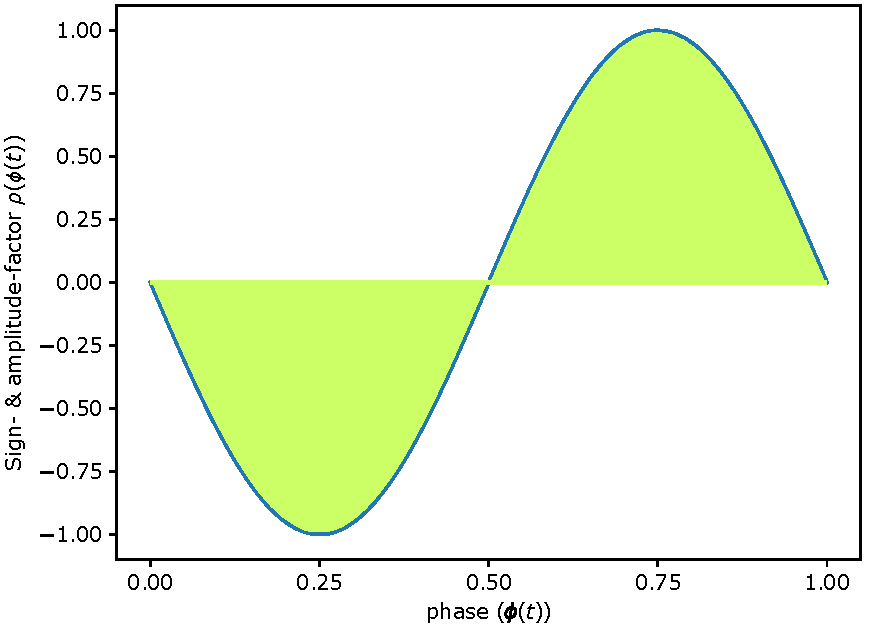
\includegraphics[width=0.65\linewidth]{Assets/DocSegments/Chapters/Baseline/Figures/Functions/all_possible_H_n_values.pdf}
		\caption[Plot of all possible frequency-adjustment contribution-values, $H(n)$-values, for K. Nymoen's frequency-adjustment]{All possible $H(n)$-values marked in green, given by $\rho(n) \cdot s(n)$, where $\rho(n)$ is defined as above and depicted in Figure \ref{fig:rho_n}, and the self-assessed synch-scores $s(n) \in [0, 1]$. The $s(n)$-scores were again simply the median of $m$ error-scores \{$\epsilon(n)$, $\epsilon(n-1)$, $\epsilon(n-2)$, ... , $\epsilon(n-m)$\} which again were given by the error-function \eqref{error_measurement} plotted in Figure \ref{fig:error_measurement}. Observe, in conjunction with Equation \eqref{freq_adj}, what the authors \cite{nymoen_synch} point out when describing their frequency update function, when saying that they specify a function that decreases frequency if a fire event is received in the first half of a node's cycle (i.e. phase $\phi(t)<0.5$), and speeds up if in the last half (to ``catch up' with the firing node). Also note how the wanted design of the authors, of causing (close to) 0 change to the frequency half-way through the cycle, is enabled by how the ``frequency-adjustment-contribution'' $H(n)$ can be equal to 0 despite the reacting node having high error scores and a high $s(n)$-score.}
		\label{fig:all_possible_H_n_values}
	\end{figure}

	To recall, the self-assessed synch-score $s(n)$ tells an adjusting agent how in- or out-of-synch it was during the last $m$ perceived ``fire''-/``flash''-events — where $s(n)=0$ signifies a mean of 0 in error-scores, and $s(n)=1$ signifies a mean of 1 in error-scores. So then if this $H$-value is to be used to adjust the nodes's frequencies with, the frequency will then be adjusted in a certain direction and amount (specified by $\rho(n)$) — given that the agent is \textit{enough} ``out of synch''/``unsynchronized'' (in the case $s(n)$ is considerably larger than 0).

	The H-value says something about how much ``out of phase'' the agent was at the time the agent's $n$th ``flashing''-signal was perceived (and then followingly how much it should be adjusted, as well as in which direction after having been multiplied together with a sign-factor $\rho(n))$, given then that this H-value also consists of the \textit{self-assessed synch score s(n)} — which again simply was the median of error-scores.

	We could look at this $H$-value as representing the direction and amplitude of the frequency adjustment weighted by the need to adjust (due to being out of synch) at the time of hearing ``fire''-/``flash''-event $n$. Or in other words, this $H$-value is then the $n$-th contribution with which we want to adjust our frequency with.

	Especially interesting cases are when we have $\phi(n)\approx0.5 \implies \rho(n)\approx\pm0$, as well as the last $m$ Error-scores $\epsilon(n)$ being close to 0, also leading to $s(n)\approx0$. In both of these two cases the entire frequency-adjustment contribution $H$ would be cancelled out, due to harmonic synchronization (legally hearing a ``fire''-/``flash''-event half-way through ones own phase) in the first case, and due to not being out of synch in the latter (having low Error-Measurements). Cancelling out the frequency adjustment contribution in these cases is then not something bad, but something wanted and something that makes sense. If these $H$-values then are cancelled out or very small, it is indicative of that nodes are already in \textit{harmonic synchrony}, and hence should not be ``adjusted away'' from this goal state. On the other side, if these $H$-values then are different (e.g. closer to -1 and 1), it is indicative of that nodes are not yet in \textit{harmonic synchrony}, and that they hence should be ``adjusted closer'' to the goal state.
	

	\paragraph{The final step: the frequency update function, $\omega_i(t^+)$}
	
		% --- META INFO START: ---
		
		\besk{ Om F(n) og selve oppdateringen av frekvens }
		
		% --- META INFO STOP. ---
	
	Now, we can pull it all together, for Nymoen et al.'s Frequency Adjustment approach for achieving harmonic synchrony with initially randomized and heterogenous frequencies.

	When an agent $i$ has a phase-climax ($\phi_i(t)=1$), it will update/adjust its frequency to the new $\omega_i(t^+)$ accordingly:

	\begin{equation}
	\label{freq_adj}
		\omega_i(t^+) = \omega_i(t) \cdot 2^{F(n)},
	\end{equation}

	where $t^+$ denotes the time-step immediately after phase-climax, and $F(n)$ is found by:

	\begin{equation}
	\label{f_value}
		F(n) = \beta\sum_{x=0}^{k-1}\frac{H(n-x)}{k},
	\end{equation}

	where $\beta$ is the frequency coupling constant, $k$ is the number of heard/received ``fire-event''s from the start of the last oscillator period to the end (i.e. the phase-climax, or \textit{now}) — and the rest of the values are as described above.

	This $F(n)$-value then, as we see in Equation \eqref{f_value}, is a weighted average of all the agent's $H(n)$-values accumulated throughout the agent's last cycle.

% --- \section END. ---



\section{System target state: harmonic synchrony}
\label{sec:harmonic_synchrony}


	% --- META INFO START: ---

	\besk{ Om target-staten til systemet, som oppfunnet av Kristian Nymoen et al. (?) }

	% --- META INFO STOP. ---


The state of harmonic synchrony is defined \cite{nymoen_synch} as the state in which all agents in the musical collective ``fire''/``flash'', as described in Subsection \ref{subsec:fire_signal}, at an even and underlying interval or pulse, a certain number of times in a row. This is not to say all agents will have to ``fire''/``flash'' simultaneously, as has traditionally been the case for pulse-coupled oscillators \cite{}. But somehow, for phases $\phi$ to be harmonically synchronized, all agent ``fire''-signals will have to coincide in a way, even though they don't all have to incur exactly at the same time always. Exactly how this looks is shown visually in Section \ref{sec:detecting_harmonic_synchrony}, especially in Figure \ref{fig:harmonic_synchrony_detection_plot}.

As one is designing and creating an interactive music technology system, one might want to encourage and allow for the playing of various musical instruments at various rhythms/paces, as it might be quite boring if all instruments were played at the exact same measure or pulse. As K. Nymoen et al. \cite{nymoen_synch} reason when discussing their own interactive ``Firefly'' music-system, as well as coining the term of \textit{harmonic synchrony}: \nl

\textit{Temporal components in music tend to appear in an integer-ratio relation to each other (e.g., beats, measures, phrases, or quarter notes, 8ths, 16ths)}. \nl

and \nl

\textit{Being an interactive music system, people may want their device to synchronize with different subdivisions of a measure (e.g. some play quarter notes while others play 8ths).} \nl

Accomodating for these aspects then, K. Nymoen et al. took inspiration for coining a novel state of synchronization for a decentralized system. This novel state arose from the concept of \textit{harmonics} in the frequency spectrum of a waveform; in that each harmonic wave or overtone has a frequency with an integer relationship to the fundamental (smallest) frequency in a waveform. Such a phenomenon, used as inspiration by Nymoen et al. but not as the basis for any definitions directly, can e.g. be seen in the frequency spectrogram of a humanly hummed G3-tone, depicted in Figure \ref{fig:sub:G3_hummed_waveform}. In said example, one can observe the presence of harmonics and overtones having frequencies with integer relationships to the fundamental (smallest) frequency at around 196 Hz, as we see the overtones e.g. has frequencies of around 400Hz, 800Hz, and 1600Hz. We will soon see how such relationships in frequency are used as inpiration for a new definition of a synchronous state; however, the example in Figure \ref{fig:frequency_spectrograms} is only meant to give an idea of where this new state of synchronization stems from, and not as a visual representation of said novel synchrony state.

\begin{figure}[ht!]
	\centering
	\begin{subfigure}[t]{.5\textwidth}
		\centering\captionsetup{width=.9\linewidth}%
		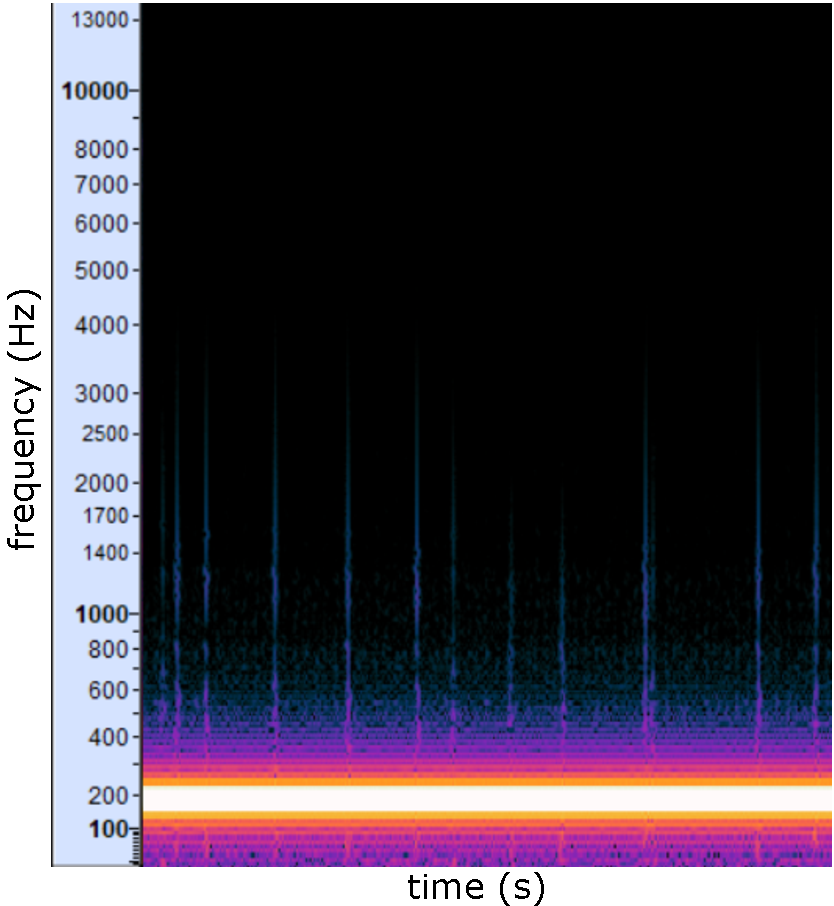
\includegraphics[width=0.9\linewidth]{Assets/DocSegments/Chapters/Baseline/Figures/Illustrations/G3_196Hz_PureTone_waveform_spectrogram.pdf}
		\caption{The frequency spectrogram of the audible waveform being a monotone and purely generated G3-tone at 195.99 Hz \cite{generate_tones}.}
		\label{fig:sub:G3_pure_waveform}
	\end{subfigure}%
	\begin{subfigure}[t]{.5\textwidth}
		\centering\captionsetup{width=.9\linewidth}%
		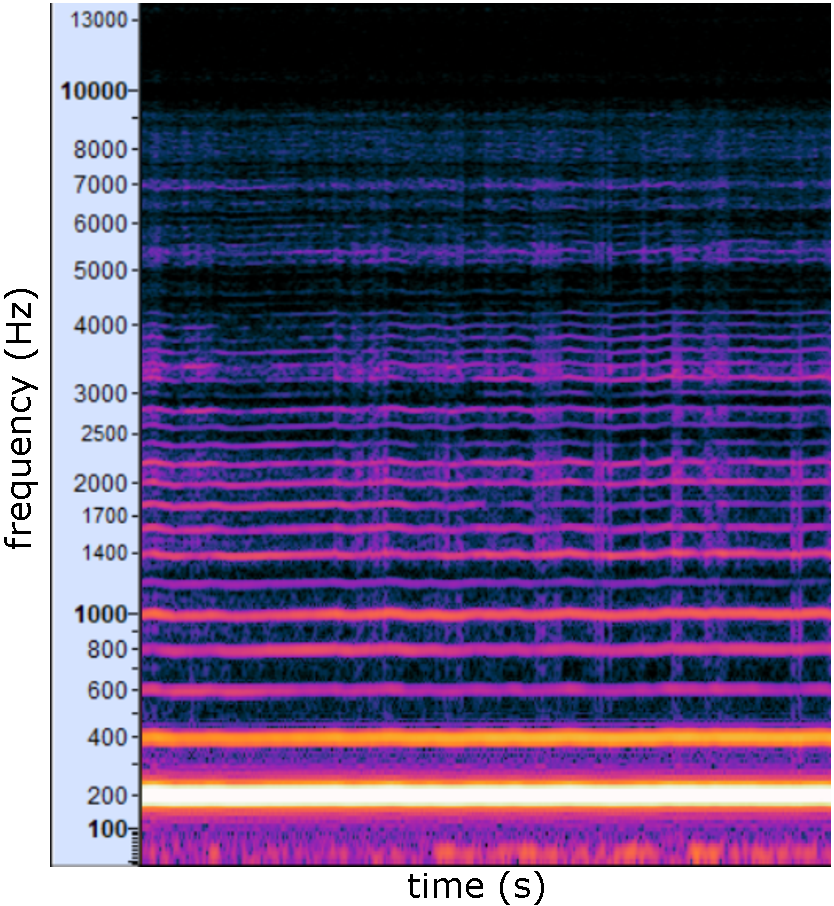
\includegraphics[width=0.9\linewidth]{Assets/DocSegments/Chapters/Baseline/Figures/Illustrations/G3_196Hz_HummingWaveform_FrequencySpectrum.pdf}
		\caption{The frequency spectrogram of the audible waveform being a more-or-less monotone but non-pure G3-tone, hummed and recorded by me \cite{}, as I tried to repeat the tone in \ref{fig:sub:G3_pure_waveform} with my voice.}
		\label{fig:sub:G3_hummed_waveform}
	\end{subfigure}
	\caption[Frequency spectrograms illustrating the absence and presence of harmonics and overtones in audible waveforms]{Frequency spectrograms of two different-sounding waveforms of the same G3-tone at 195.99 Hz. Note the absence and presence of harmonics and overtones in waveform \ref{fig:sub:G3_pure_waveform} and \ref{fig:sub:G3_hummed_waveform} respectively, as well as the integer-relationships between the fundamental (lowest) frequency and the harmonics in \ref{fig:sub:G3_hummed_waveform}. Frequencies in a harmonically synchronized agent collective will for the first $\phi$-problem resemble the frequencies in \ref{fig:sub:G3_pure_waveform}, where all frequencies are equal and constant. Conversely, when frequencies can be heterogenous and unequal, as in the $\phi$- \& $\omega$-problem, the frequencies in a harmonically synchronized agent collective will rather resemble, although not completely correspond to, the frequencies in \ref{fig:sub:G3_hummed_waveform}, where higher frequencies with integer relationships to the fundamental and lowest frequency can be present at the same time.}
	\label{fig:frequency_spectrograms}
\end{figure}

More accurately then and inspired by integer relationships in waveforms, although not exactly analogus to the example above in Figure \ref{fig:frequency_spectrograms}, Nymoen et al. describe \textit{legal} frequencies the oscillator frequencies has to lie within to be considered \textit{harmonically synchronized}: \nl

\textbf{Legal frequencies definition:} \nl

All musical robots $i$, in a harmonically synchronized state, will have oscillator frequencies $\omega_i$ which are element in the mathematical set

\begin{equation}\label{legal_freqs}
\Omega_{legal}(\omega_0) = \omega_{0} \cdot 2^{\mathbb{N}_0} = \{\omega_{0}, 2\omega_{0}, 4\omega_{0}, 8\omega_{0}, ...\} ,
\end{equation}

where $\omega_{0}$ is the lowest frequency in the robot-collective (or the fundamental frequency if you will), and $\mathbb{N}_0$ are the natural numbers including the number zero. \nl

If e.g. the smallest oscillator frequency in the musical robot collective ($\omega_0$) was equal to 1.5Hz, \textit{legal} oscillator frequencies the rest of the musical robots in the collective could have would be $\Omega_{legal}$(1.5Hz) = \{1.5Hz, 3Hz, 6Hz, 12Hz, ...\}.

Hence, in terms of oscillator frequencies $\omega_i$ for all robots $i$ in the musical robot collective, we have \textit{harmonically synchronized} and \textit{legal} oscillator frequencies $\omega_i$ if (and only if)

\begin{equation}\label{synced_freqs}
\omega_i \in \Omega_{legal}(\omega_0) , \forall i.
\end{equation} \nl

Note that the only difference between this definition of \textit{legal oscillator frequencies} and the spectrogram example depicted in Figure \ref{fig:frequency_spectrograms} lies in that for the legal frequencies as defined in \eqref{legal_freqs}, higher frequencies can only have doubling integer relationships with the lowest fundamendal frequency (e.g. twice or four times as high), whereas the frequencies of the harmonics seen in the humanly hummed G3 tone (\ref{fig:sub:G3_hummed_waveform}) additionally had all other positive integer relationships (e.g. three or five times as high) with the fundamental frequency.

This state of \textit{harmonic synchrony} is then the system goal state K. Nymoen et al. achieve using their phase and frequency update functions, as explained above in Section \ref{nymoen_phase_adjust} and \ref{nymoen_freq_adjust}; and is also the target or goal state we want to continue achieving and experimenting for in this thesis.


	\subsection{Detecting harmonic synchrony}
	\label{subsec:harmonic_synchrony}
	In order to test and evaluate synchronization performance in their firefly-inspired oscillator-system, K. Nymoen et al. \cite{nymoen_synch} develop a measurement used to detect when the system has reached a state of synchrony. Using the firings of the fireflies, some well-defined conditions have to be met in order for the fireflies to be deemed \textit{harmonically synchronized}: \nl
	
	\textbf{Harmonic synchronizaton conditions:}
	
	\begin{itemize}
		\item[] \textbf{Condition 1}: Firing may only happen within a short time period $t_f$.
		\item[] \textbf{Condition 2}: All nodes must have fired at least once during the evaluation period.
		\item[] \textbf{Condition 3}: Between each $t_f$, a period $t_q$ without fire events must be equally long $k$ times in a row.
	\end{itemize}
	\sep
	
	By utilizing transmitted firings/pulses from the robots in our robot-collective, these conditions can be enforced and checked throughout the synchronization-process, in order to detect if the oscillator-network becomes harmonically synchronized.
	
	For getting a better idea of how these conditions being met looks like, see the \textbf{Harmonic synchrony detection plot} in Figure \ref{fig:harmonic_synchrony_detection_plot} where the oscillators/robots fulfill the abovementioned requirements right before ending the synchronization process.
	
	These requirements, amongst other illustrations in Nymoen et al.'s paper \cite{nymoen_synch}, thus constitutes a blueprint for the design of a performance or synchrony measurement able to detect the achievement of harmonic synchrony in a decentralized network of ``firing''—or pulse-coupled—oscillators. The time having passed from the start of the synchronization-process until the detection of harmonic synchrony will then be defined as the performance score, indicating how fast or slow the oscillators are at synchronizing.
	
	The exact details of how such a performance or synchrony measurement is implemented for our musical multi-robot oscillator-network, in the synchronization-simulator, will be given in Section \ref{sec:detecting_harmonic_synchrony}.
	
% --- \section END. ---